%%%%%%%%%%%%%%%%%%%%%%%%%%%%%%%%%%%%%%%%%
% fphw Assignment
% LaTeX Template
% Version 1.0 (27/04/2019)
%
% This template originates from:
% https://www.LaTeXTemplates.com
%
% Authors:
% Class by Felipe Portales-Oliva (f.portales.oliva@gmail.com) with template 
% content and modifications by Vel (vel@LaTeXTemplates.com)
%
% Template (this file) License:
% CC BY-NC-SA 3.0 (http://creativecommons.org/licenses/by-nc-sa/3.0/)
%
%%%%%%%%%%%%%%%%%%%%%%%%%%%%%%%%%%%%%%%%%

%----------------------------------------------------------------------------------------
%	PACKAGES AND OTHER DOCUMENT CONFIGURATIONS
%----------------------------------------------------------------------------------------

\documentclass[
	12pt, % Default font size, values between 10pt-12pt are allowed
	%letterpaper, % Uncomment for US letter paper size
	%spanish, % Uncomment for Spanish
]{fphw}

% Template-specific packages
\usepackage[utf8]{inputenc} % Required for inputting international characters
\usepackage[T1]{fontenc} % Output font encoding for international characters
\usepackage{mathpazo} % Use the Palatino font
\usepackage[dvipsnames]{xcolor}
\usepackage{graphicx} % Required for including images
\usepackage{amsmath}
\usepackage{booktabs} % Required for better horizontal rules in tables
\usepackage{listings} % Required for insertion of code
\usepackage{enumerate} % To modify the enumerate environment
\usepackage{ragged2e}
\usepackage{cancel}
\usepackage{MnSymbol,bbding,pifont}
\usepackage{lscape}
\usepackage{array}
\usepackage{float,graphicx}
\newcolumntype{M}{>{$}c<{$}}
%----------------------------------------------------------------------------------------
%	ASSIGNMENT INFORMATION
%----------------------------------------------------------------------------------------

\title{Assignment \#1} % Assignment title

\author{Luis Alberto Ballado Aradias} % Student name

\date{\today} % Due date

\institute{Centro de Investigación y de Estudios Avanzados del IPN \\ Unidad Tamaulipas} % Institute or school name

\class{Tecnologías Computacionales (Sep - Dec 2022)} % Course or class name

\professor{Dr. Edwin Aldana Bobadilla} % Professor or teacher in charge of the assignment

%----------------------------------------------------------------------------------------

\begin{document}

\maketitle % Output the assignment title, created automatically using the information in the custom commands above

%----------------------------------------------------------------------------------------
%	ASSIGNMENT CONTENT
%----------------------------------------------------------------------------------------

%------------------------------------------------



\begin{enumerate}
\item Diseñar autómatas finitos deterministas que acepten los siguientes lenguajes:
  \begin{enumerate}[(i)]
  \item $\Sigma = \left\lbrace0,1\right\rbrace$ , $L= $ lenguaje de las cadenas sobre $\Sigma$ de longitud impar.\\
    
  \item $\Sigma = \left\lbrace 0,1 \right\rbrace$ , $L= $ lenguaje de las cadenas sobre $\Sigma$ que contienen un número impar de unos.\\
    
  \item $\Sigma = \left\lbrace a,b \right\rbrace$ , $L= ab^{+}$ \\
    
  \item $\Sigma = \left\lbrace a,b \right\rbrace$ , $L= ab^{*} \cup ab^{*}a$ \\
    
  \item $\Sigma = \left\lbrace 0,1 \right\rbrace$ , $L= \left(0 \cup 10\right)^{*} $ \\
    
  \item $\Sigma = \left\lbrace 0,1 \right\rbrace$ , $L= \left(01 \cup 10\right).^{*}$ \\

  \item $\Sigma = \left\lbrace 0,1 \right\rbrace$ , Lenguaje de todas las cadenas que no contienen dos unos consecutivos. \\
  \item $\Sigma = \left\lbrace a,b \right\rbrace$ , $L= \left\lbrace a^{2i} b^{3j} : i,j \geq 0 \right\rbrace$ \\
  \item $\Sigma = \left\lbrace a,b \right\rbrace$ , $L= $ lenguaje de las cadenas sobre $\Sigma$ que contienen un número par de $aes$ y un número par de bes. Ayuda: utilizar 4 estados.\\
  \item $\Sigma = \left\lbrace a,b \right\rbrace$ . Para cada combinación de las condiciones "par" e "impar" y de las conectivas "o" e "y", diseñar un AFD que acepte el lenguaje $L$ definido por\\
    $L= $ lenguaje de las cadenas con un número par/impar de aes y/o un número par/impar de bes.\\
    Ayuda: utilizar el autómata de 4 estados diseñado en el ejercicio anterior, modificado adecuadamente el conjunto de estados finales.
  \end{enumerate}
\end{enumerate}

%------------------------------------------------


\begin{enumerate}
  \setcounter{enumi}{1}
\item Determinar los lenguajes aceptados por los siguientes AFD. Describir los lenguajes ya sea por medio de una propiedad característica o de una expresión regular.
  \begin{enumerate}[i]
  \item uno\\
    \begin{figure}[H]
      \centering
      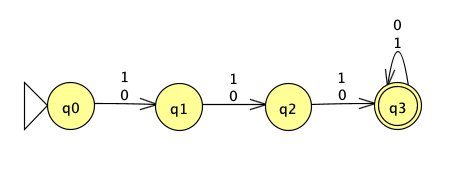
\includegraphics[width=\linewidth]{images/graph1.png}
    \end{figure}
  \item dos\\
    \begin{figure}[H]
      \centering
      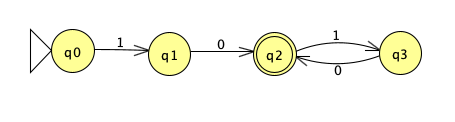
\includegraphics[width=\linewidth]{images/graph2.png}
    \end{figure}
  \item tres\\
    \begin{figure}[H]
      \centering
      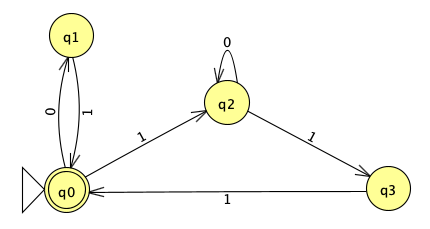
\includegraphics[width=\linewidth]{images/graph3.png}
    \end{figure}
  \item cuatro\\
    \begin{figure}[H]
      \centering
      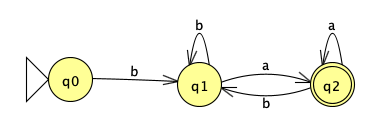
\includegraphics[width=\linewidth]{images/graph4.png}
    \end{figure}
  \end{enumerate}

\end{enumerate}
%----------------------------------------------------------------------------------------


\end{document}
